\usetikzlibrary{calc}


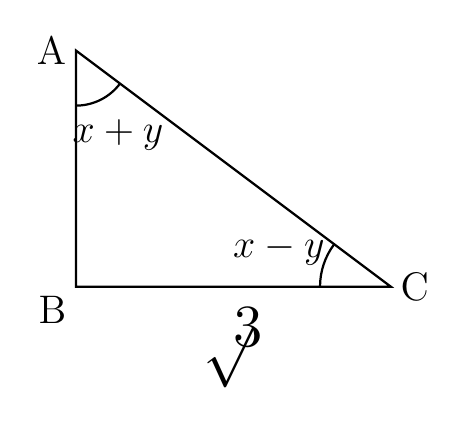
\begin{tikzpicture}[scale=1, every node/.style={font=\Large}]

    % Define the vertices of the right-angled triangle
    \coordinate (B) at (0,0);
    \coordinate (C) at (4,0);
    \coordinate (A) at (0,3);

    % Draw the triangle
    \draw[thick] (A) -- (B) -- (C) -- cycle;

    % Draw the angle arcs
    % Angle A (starts from AB straight down at 270° to AC at 323.13°)
    \draw[thick] (0, 2.3) arc (270:323.13:0.7);
    \node at ($(A) + (296.5:1.2)$) {$x+y$};

    % Angle C (starts from CB straight left at 180° to CA at 143.13°)
    \draw[thick] (3.1, 0) arc (180:143.13:0.9);
    \node at ($(C) + (161.5:1.5)$) {$x-y$};

    % Add labels for the vertices
    \node[left] at (A) {A};
    \node[below left] at (B) {B};
    \node[right] at (C) {C};

    % Add length label for side BC
    % \raisebox{-6.5pt} pulls the \surd symbol even further downwards relative to the 3
    \node[below, yshift=-4pt] at (2,0) {\scalebox{1.5}{\raisebox{-6.5pt}{$\surd$}$\!\!3$}};

\end{tikzpicture}